\section{Introduction}
\label{section:introduction}




The database, HCI and systems communities have proposed an excess of tools that manage to simplify common tasks that typically take place in an analytical process. Such tools, however, either tend to focus on only individual stages (such as data retrieval or visualization) of a much bigger analytical pipeline or while they do provide a bigger set of possible operations, they only focus on particular use cases (for instance pattern matching, finding correlations and so on)\costas{todo: add references}. Despite the remarkable contributions, data scientists often have to combine such tools in order to complete an analysis. This lack of flexibility often pushes code-literate data scientists to the tested and proven path of interactive notebooks such as Jupyter.

Interactive notebooks allow the use of popular, high-level and highly expressive imperative languages, such as Python, for retrieving, processing and visualizing data, all in one platform. Due to the high popularity of the languages they support, there is also a massive collection of utility libraries that can be used to facilitate any potential data science project. Furthermore, the web environment of notebooks enables collaboration between data scientists, since it allows them to develop and run code that processes data and generates visualizations directly on the browser. Lastly, after completing an analysis, data scientists can compose their findings into an interactive report-like page, that contains re-runnable code, visualizations and textual description of the analysis, which can also be shared with non-technical users. \costas{maybe add a small figure of the jupyter UI?}For those reasons, notebooks are extensively used in data science projects.

\eat{
Additionally, the notebook-like interface, they offer, enables the creation of interactive documents that contain code, textual description and visualizations, which helps readers follow the analysis and perhaps re-run certain blocks of that notebook.



. Due to the wide popularity of such languages, there is also a huge collection of third-party libraries that can be used by data scientists as building blocks of a much bigger analytical process. Furthermore, the web environment of notebooks enables collaboration between data scientists, since it allows them to directly interact with the user interface in order to develop and run code, process data, generate visualizations, and lastly, compose their findings into an interactive (and re-runnable) report-like page, that contains code, visualizations and textual description of the analysis.
}
However as we show in this work, interactive notebooks are still suboptimal with regard to ease of use for data analysts. Retrieving, processing and visualizing data requires technical expertise that often exceeds the skill-set of a typical data scientist. Specifically, such steps require data transfers and package installations on the notebook server, in order to be used in an analysis. Such tasks fit the job description of a system administrator rather than a data analyst. Additionally, even after the environment has been setup, the data analyst has to read long documentation files that explain how to programmatically interact with such tools and she often has to spend significant effort writing plumbing code in order combine their functionality.




Other than the aforementioned limitations that mainly impact data analysts, notebooks also have limitations that impact the, potentially non-technical, readers of the generated notebooks. Particularly, while notebooks can contain visualizations that showcase important aspects of a data analysis, the readers cannot interact with the provided visualizations in the same way they could if these visualizations were part of a dashboard application. Specifically, even if the analyst that composed the notebook used third-party web-based visualization libraries that allow some user interaction, this interaction is limited to individual changes occurring only to the visualization with which the reader  interacts and cannot trigger changes to other parts of the notebook. For this reason, only code-literate readers, capable of extending the notebook with more coding snippets, are able to further explore the underlying data, while the rest are limited to passively reading the generated notebook.\\




\noindent {\bf Contributions.}
In order to resolve these issues, we extend interactive notebooks with the  {\projname} notebook engine. The main contributions of this extension are: (a) visual and data retrieval constructs, that simplify the process of data retrieval and visualization, for data analysts, (b) A declarative template language that can be used for describing computation, data transformations and user input collection, (c) A propagation algorithm, that utilizes visual and data retrieval constructs, combined with templates in order to introduce a reactive behavior in notebooks, thus enabling non-technical readers to further explore data, without requiring any coding skills. 

\eat{
The remainder of this paper is organized as follows: Section ?? discusses the architecture of the {\projname} framework. Due to space limitation, we focus on those aspects that can be useful as a notebook extension. Section ?? presents our example data analysis. Finally, Section ?? concludes the paper.
}

\eat{
\noindent {\bf Contributions.}
To sum up, we extend interactive notebooks with the  {\projname} notebook engine. The main contributions of this extension are: (a) visual and data retrieval constructs, that simplify the process of data retrieval and visualization, (b) A declarative template language that can be used for specifying computation, data transformations and user input collection, (c) A propagation algorithm, that utilizes visual and data retrieval constructs, in association with a template language in order to introduce a reactive in notebooks. 
}
\eat{

\begin{itemize}
	\item \textit{Expressive template language:} Prior work, treats a page as a database view. Building on that, our template language goes beyond SQL query and view definition in both style and fundamental expressiveness. It is a mixture of query as well as web templating language that works on ordered (arrays) and semi-ordered (JSON) data. 
	\item \textit{Easy data retrieval:} Our framework supports communication with all major database types, such as Postgress, MongoDB, SQL etc, eliminating the need for individual DB drivers. Furthermore, using {\projname}, user access credentials for the database server(s) are stored in a configuration file, eliminating the embarassingly insecure practice of typing usernames and passwords in notebook cells vidible to everyone.
	\item \textit{Inline JSON operations:} The primary data structure used in {\projname} is JSON arrays. {\projname} combines the intuitive nature of JSON with the ability to write inline JSON operations, resulting in a clean, structured and readable code.
	\item \textit{Variable binding:} Analysts can easily ``bind'' variables using our template language. ``Binding'', results in automatic re-execution of notebook cells that contain those variables upon a change. {\projname} will trigger execution of the appropriate cells without any extra coding effort. As we show later, combined with inline JSON operations, binding becomes an incredibly versatile tool.

%	\item \textit{Declarative semantics:} {\projname} implements formal declarative \textit{Model-View-View-Model} (MVVM) semantics. \remark{Fill in why this is a good thing. I have no idea.}
%	\item \textit{Expressive template language:} Prior database work, treats a page as a database view. Building on that, our template language goes beyond SQL query and view definition in both style and fundamental expressiveness. It is a mixture of query as well as web templating language that works on ordered (arrays) and semi-ordered (JSON) data. 
%	\item We allow in-line declarative code directly in JSON...
\end{itemize}

}


\eat{
\begin{figure*}
	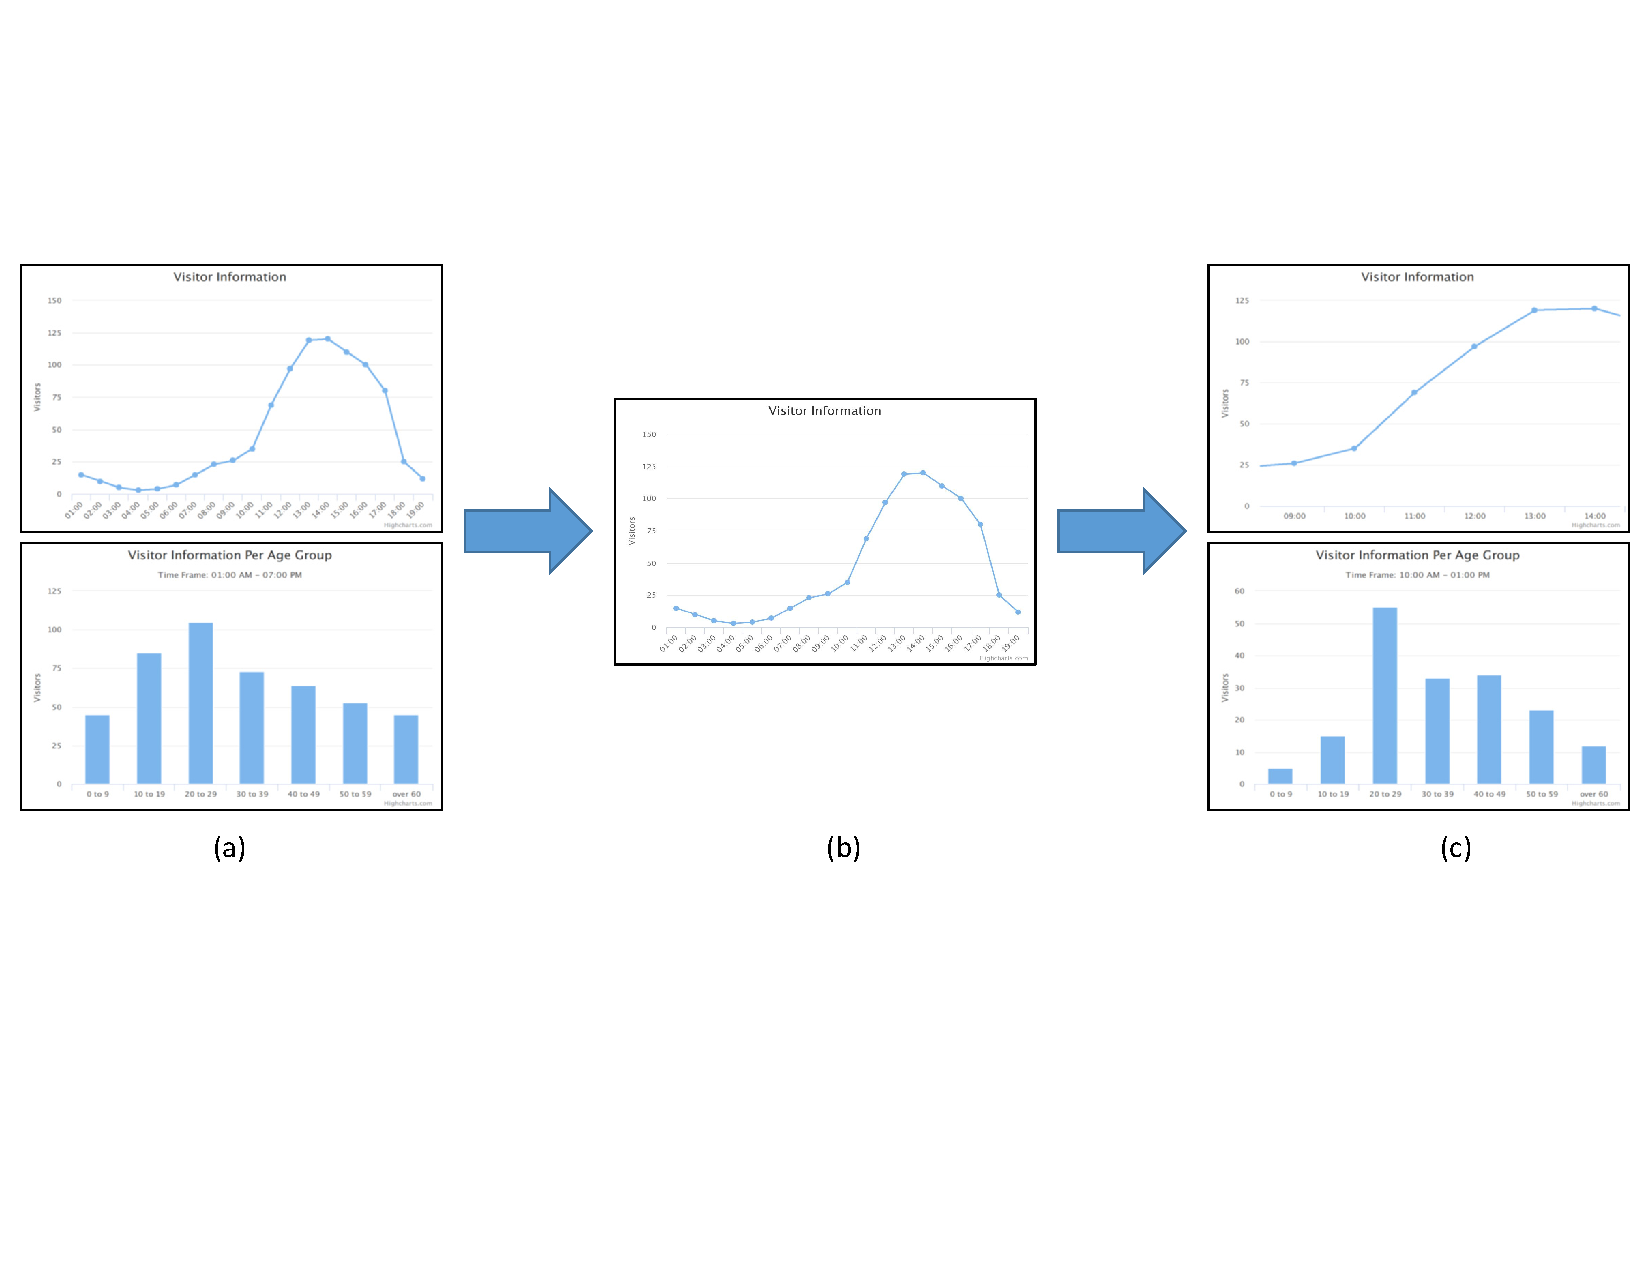
\includegraphics[width=\textwidth]{figures/highchart_final_a.pdf}
	\caption{Demonstration of interactive charts. The analyst's selection automatically updates the second plot (right).}
	\label{fig:vision}
\end{figure*}
}
\eat{
\begin{figure*}
	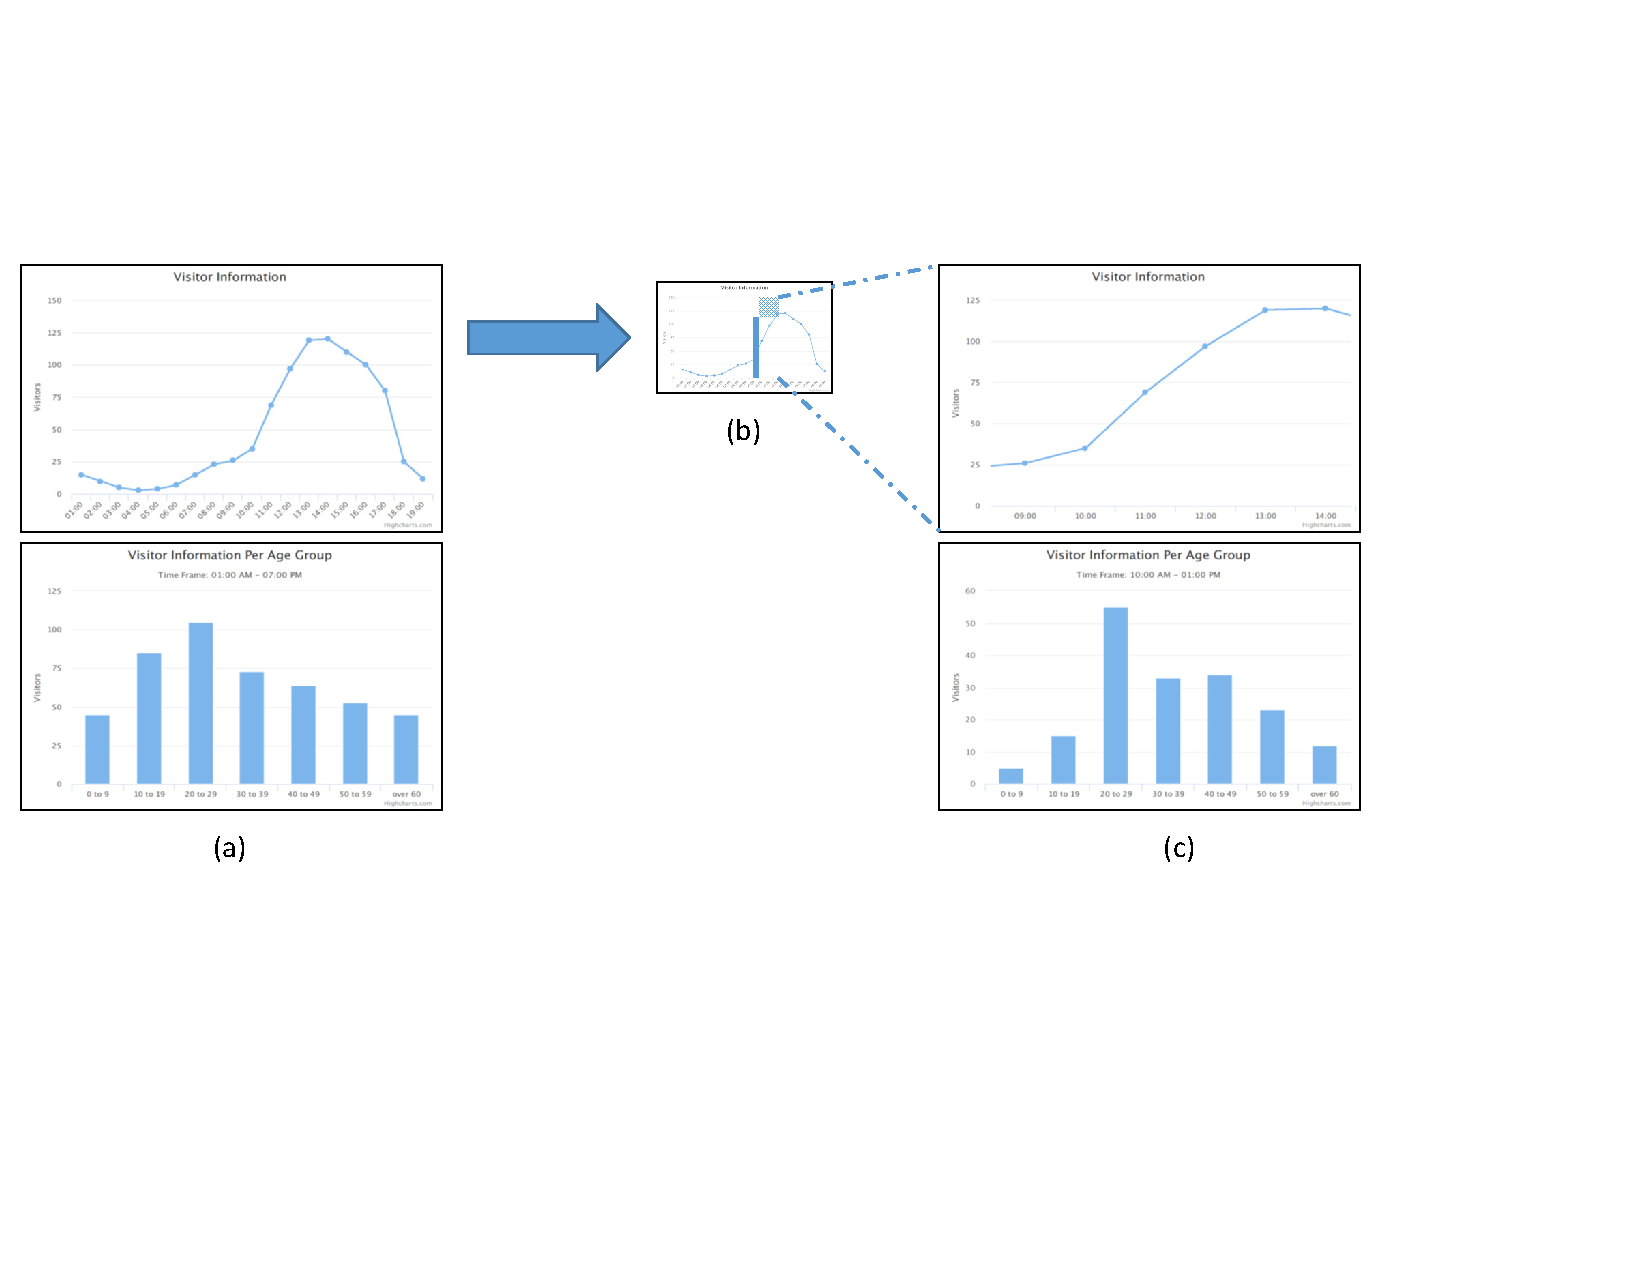
\includegraphics[width=\textwidth]{figures/highchart_final_b.pdf}
	\caption{Demonstration of interactive charts. The analyst's selection automatically updates the second plot (right).}
	\label{fig:vision}
\end{figure*}
}
\eat{
\remark{Ok I thought about it and I propose the following modifications in the paper structure (Nothing major - just moving text around to make it more readable): We begin with a good discussion about the vidette features that can help notebooks in section 2. We then show the entire walkthrough in one section (Section 3). By now, the reader knows what vidette can do so it will be easier to follow and understand the code we show.}
}
 \eat{
We address these issues, by extending interactive notebooks with the  {\projname} framework. {\projname} notebooks support a new template language capable of facilitating common data analysis tasks. The main contributions of this extension are:

\begin{itemize}
	\item \textit{Expressive template language:} Prior work, treats a page as a database view. Building on that, our template language goes beyond SQL query and view definition in both style and fundamental expressiveness. It is a mixture of query as well as web templating language that works on ordered (arrays) and semi-ordered (JSON) data. 
	\item \textit{Easy data retrieval:} Our framework supports communication with all major database types, such as Postgress, MongoDB, SQL etc, eliminating the need for individual DB drivers. Furthermore, using {\projname}, user access credentials for the database server(s) are stored in a configuration file, eliminating the embarassingly insecure practice of typing usernames and passwords in notebook cells vidible to everyone.
	\item \textit{Inline JSON operations:} The primary data structure used in {\projname} is JSON arrays. {\projname} combines the intuitive nature of JSON with the ability to write inline JSON operations, resulting in a clean, structured and readable code.
	\item \textit{Variable binding:} Analysts can easily ``bind'' variables using our template language. ``Binding'', results in automatic re-execution of notebook cells that contain those variables upon a change. {\projname} will trigger execution of the appropriate cells without any extra coding effort. As we show later, combined with inline JSON operations, binding becomes an incredibly versatile tool.

%	\item \textit{Declarative semantics:} {\projname} implements formal declarative \textit{Model-View-View-Model} (MVVM) semantics. \remark{Fill in why this is a good thing. I have no idea.}
%	\item \textit{Expressive template language:} Prior database work, treats a page as a database view. Building on that, our template language goes beyond SQL query and view definition in both style and fundamental expressiveness. It is a mixture of query as well as web templating language that works on ordered (arrays) and semi-ordered (JSON) data. 
%	\item We allow in-line declarative code directly in JSON...
\end{itemize}
}


%In this paper, we demonstrate the use of {\projname} via a walkthrough example. Specifically, we want to use website access data to plot an access count over time histogram. We also want to plot the recorded user demographics (with focus on age groups). We then want to have the ability to interact with the histogram plot and select a time region. This action should automatically update the second plot with the user demographics in the selected time window. 
%
%Without loss of generality, we assume a Jupyter server, where the analysts develop their notebooks and a different database server where data is stored. To retrieve the entirety of the required data, we have to query two different databases and join the returned JSON files. Figure ?? shows how our databases are organized. Our fictional analyst will perform the following high-level tasks:
%
%\begin{itemize}
%	\item Data retrieval from remote databases. 
%	\item Data curation: Join data and prepare for visualization.
%	\item Data visualization.
%\end{itemize}
%
%The remainder of this paper is organized as follows: Sections \ref{section:dataretrieval} -- \ref{section:visualization} present a direct comparison of using {\projname} and an imperative language such as Python in order to complete the tasks of our example. Throughout these sections, we demonstrate some of the main contributions of {\projname}. Section \ref{section:discussion} provides further discussion regarding our proposed extension and presents other useful aspects of it not used in our walkthrough. Finally, Section \ref{section:conclusion} concludes the paper.

